\documentclass[review,supplement,onefignum,onetabnum]{siamart190516}
%\usepackage[colorlinks=true,urlcolor=blue,citecolor=blue,linkcolor=blue]{hyperref}
\usepackage[linesnumbered, ruled, vlined, algo2e]{algorithm2e}
%\usepackage{natbib}
%\usepackage[sort]{cite}
\pdfoutput=1
%\usepackage[colorlinks=true,urlcolor=blue,citecolor=blue,linkcolor=blue]{hyperref}
\usepackage[english]{babel}
\usepackage[utf8]{inputenc}
\usepackage[T1]{fontenc}
\usepackage{amssymb}
\usepackage{tabularx}
\usepackage{quoting}
\usepackage{upquote}
\usepackage{subcaption}
\usepackage{multicol}
\usepackage{cancel}
\usepackage[framemethod=TikZ]{mdframed}
\usetikzlibrary{shapes}
\usetikzlibrary{snakes}
\usetikzlibrary{shapes.geometric}
\usepackage{wrapfig}
%\usepackage{caption}
%\usepackage[plain]{algorithmic}
\usepackage{algpseudocode}
\usepackage{rotating}
%\usepackage{cite}
\usepackage{booktabs}
%\usepackage{unicode-math}
%\usepackage{algorithm}% http://ctan.org/pkg/algorithm
%\usepackage{algpseudocode}% http://ctan.org/pkg/algpseudocode
\usepackage{xcolor}% http://ctan.org/pkg/xcolor
\makeatletter
\newsavebox{\@brx}
\newcommand{\llangle}[1][]{\savebox{\@brx}{\(\m@th{#1\langle}\)}%
  \mathopen{\copy\@brx\kern-0.5\wd\@brx\usebox{\@brx}}}
\newcommand{\rrangle}[1][]{\savebox{\@brx}{\(\m@th{#1\rangle}\)}%
  \mathclose{\copy\@brx\kern-0.5\wd\@brx\usebox{\@brx}}}
\makeatother
\usepackage{bbm}
\usepackage{jlcode}
\usepackage{graphicx}
\usepackage{amsmath,color}
\usepackage{mathrsfs}
\usepackage{float}
\usepackage[normalem]{ulem}
\usepackage{makecell}
\usepackage{indentfirst}
\usepackage{txfonts}
%\usepackage[epsilon, tsrm, altpo]{backnaur}

\makeatletter
\def\parsept#1#2#3{%
    \def\nospace##1{\zap@space##1 \@empty}%
    \def\rawparsept(##1,##2){%
        \edef#1{\nospace{##1}}%
        \edef#2{\nospace{##2}}%
    }%
    \expandafter\rawparsept#3%
}
\makeatother
\DeclareMathAlphabet{\mymathbb}{U}{BOONDOX-ds}{m}{n}
\newcommand{\listingcaption}[1]%
{%
\refstepcounter{lstlisting}\hfill%
Listing \thelstlisting: #1\hfill%\hfill%
}%
\newcolumntype{b}{X}
\newcolumntype{s}{>{\hsize=.7\hsize}X}
\usepackage{listings}
\lstset{
    language=Julia,
    basicstyle=\ttfamily\scriptsize,
    numberstyle=\scriptsize,
    % numbers=left,
    backgroundcolor=\color{gray!7},
    %backgroundcolor=\color{white},
    %frame=single,
    xleftmargin=2em,
    tabsize=2,
    rulecolor=\color{black!15},
    %title=\lstname,
    escapeinside={(*}{*)},
    breaklines=true,
    %breakatwhitespace=true,
    %framextopmargin=2pt,
    %framexbottommargin=2pt,
    frame=bt,
    extendedchars=true,
    inputencoding=utf8,
    columns=fullflexible,
    %escapeinside={(*@}{@*)},
}

\tolerance=1
\emergencystretch=\maxdimen
\hyphenpenalty=1000
\hbadness=1000

\makeatletter

%%%%%%%%%%%%%%%%%%%%%%%%%%%%%% User specified LaTeX commands.

%Journal reference.  Comma sets off: name, vol, page, year
\def\journal #1, #2, #3, 1#4#5#6{{\sl #1~}{\bf #2}, #3 (1#4#5#6) }
\def\pr{\journal Phys. Rev., }
\def\prb{\journal Phys. Rev. B, }
\def\prl{\journal Phys. Rev. Lett., }
\def\pl{\journal Phys. Lett., }
%\def\np{\journal Nucl. Phys., }


%%%%%%%%%%%%%%%%%%%%%%%%%%%%%%%%%%%%%%%%%%%%%%%%%%%%%%%%%%%%%%%%%%%%%%%%%%%%%%%%%%%%%%%%%%%%%%%%%%%%%%%%%%%%%%%%%%%%%%%%%%%%%%%%%%%%%%%%%%%%%%%%%%%%%%%%%%%%%%%%%%%%%%%%%%%%%%%%%%%%%%%%%%%%%%%%%%%%%%%%%%%%%%%%%%%%%%%%%%%%%%%%%%%%%%%%%%%%%%%%%%%%%%%%%%%%


%\usepackage[colorlinks, citecolor=blue]{hyperref}
\DeclareMathOperator*{\argmax}{arg\,max}

\newcommand{\eqname}[1]{\stepcounter{equation}\tag{\theequation : #1}}
%%%%%% Shortcut related
\newcommand{\<}{\langle}
\renewcommand{\>}{\rangle}
\newcommand{\out}{{\vx^L}}
\newcommand{\inp}{{\vx^0}}
\newcommand{\cquad}{{{ }_{\quad}}}
\newcommand{\pluseq}{\mathrel{+}=}
\newcommand{\minuseq}{\mathrel{-}=}
\newcommand{\vx}{{\mathbf{x}}}
\newcommand{\vg}{{\mathbf{g}}}
\newcommand{\vp}{{\mathbf{p}}}
\newcommand{\vy}{{\mathbf{y}}}
\newcommand{\Var}{{\mathrm{Var}}}
\newcommand{\Mean}{{\mathrm{E}}}
\newcommand{\vvalue}{{\texttt{value}}}
\newcommand{\grad}{{\texttt{grad}}}
\newcommand{\parameter}{{\texttt{parameter}}}
%%%%%% Convention related
\newcommand{\SWAP}{{\rm SWAP}}
\newcommand{\CNOT}{{\rm CNOT}}
\newcommand{\bigO}{{\mathcal{O}}}
\newcommand{\X}{{\rm X}}
\renewcommand{\H}{{\rm H}}
\newcommand{\Rx}{{\rm Rx}}
\renewcommand{\v}[1]{{\bf #1}}
\newcommand{\dataset}{{\mathcal{D}}}
\newcommand{\wfunc}{{\psi}}
\newcommand{\SU}{{\rm SU}}
\newcommand{\UU}{{\rm U}}
\newcommand{\thetav}{{\boldsymbol{\theta}}}
\newcommand{\gammav}{{\boldsymbol{\gamma}}}
\newcommand{\thetai}{{\theta^\alpha_l}}
\newcommand{\Expect}{{\mathbb{E}}}
\newcommand{\Tr}{{\rm Tr}}
\newcommand{\etc}{{\it etc~}}
\newcommand{\etal}{{\it etal~}}
\newcommand{\xset}{\mathbf{X}}
\newcommand{\fl}{\texttt{fl}}
\newcommand{\pdata}{\mathbf{\pi}}
\newcommand{\q}{\mathbf{q}}
\newcommand{\epdata}{\mathbf{\hat{\pi}}}
\newcommand{\gammaset}{\boldsymbol{\Gamma}}
\newcommand{\ei}{{\mathbf{e}_l^\alpha}}
\newcommand{\vtheta}{{\boldsymbol{\theta}}}
\newcommand{\sigmag}{{\nu}}
\newcommand{\sigmai}[2]{{\sigma^{#2}_{#1}}}
\newcommand{\qi}[1]{{q^{\alpha_{#1}}_{#1}}}
\newcommand{\BAS}{Bars-and-Stripes}
\newcommand{\circled}[1]{\raisebox{.5pt}{\textcircled{\raisebox{-.9pt} {#1}}}}
\newcommand{\qexpect}[1]{{\left\langle #1\right\rangle}}
\newcommand{\expect}[2]{{\mathop{\mathbb{E}}\limits_{\substack{#2}}\left[#1\right]}}
\newcommand{\var}[2]{{\mathop{\mathrm{Var}}\limits_{\substack{#2}}\left(#1\right)}}
\newcommand{\pshift}[1]{{p_{\thetav+#1}}}
\newcommand{\upcite}[1]{\textsuperscript{\cite{#1}}}
\newcommand{\bra}[1]{\mbox{$\left\langle #1 \right|$}}
\newcommand{\ket}[1]{\mbox{$\left| #1 \right\rangle$}}
\newcommand{\braket}[2]{\mbox{$\left\langle #1 | #2 \right\rangle$}}
\newcommand{\tr}[1]{\mathrm{tr}\mbox{$\left[ #1\right]$}}

\newcommand{\ra}[1]{\renewcommand{\arraystretch}{#1}}

%%%%%% Comment related
\newcommand{\red}[1]{[{\bf  \color{red}{ST: #1}}]}
\newcommand{\xred}[1]{[{\bf  \color{red}{\sout{ST: #1}}}]}
\newcommand{\green}[1]{[{\bf  \color{green}{XG: #1}}]}
\newcommand{\xgreen}[1]{[{\bf  \color{green}{\sout{XG: #1}}}]}
\newcommand{\blue}[1]{[{\bf  \color{blue}{JG: #1}}]}
\newcommand{\xblue}[1]{[{\bf  \color{blue}{\sout{JG: #1}}}]}
\newcommand{\cyan}[1]{[{\bf  \color{cyan}{ML: #1}}]}
\newcommand{\xcyan}[1]{[{\bf  \color{cyan}{\sout{ML: #1}}}]}
\newcommand{\purple}[1]{[{\bf  \color{purple}{MC: #1}}]}
\newcommand{\xpurple}[1]{[{\bf  \color{purple}{\sout{MC: #1}}}]}
\newcommand{\material}[1]{\iffalse[{\bf  \color{cyan}{Material: #1}}]\fi}

\newcounter{example}
\newenvironment{example}[1][]{\refstepcounter{example}\par\medskip
   \noindent \textbf{Example~\theexample. #1} \rmfamily}{\medskip}

%\newtheorem{theorem}{\textit{Theorem}}
%\newtheorem{corollary}{\textit Branching Rule}
%\theoremstyle{definition}\newtheorem{definition}{\textit{Definition}}
%\newtheorem{defin}[thm]{Definition}

\makeatother

\author{
Jin-Guo Liu\thanks{Department of Physics, Harvard University, Cambridge, Massachusetts 02138, USA; QuEra Computing Inc., 1284 Soldiers Field Road, Boston, MA, 02135, USA  %\thanks{QuEra Computing Inc., 1284 Soldiers Field Road, Boston, MA, 02135, USA}
    (\email{jinguoliu@g.harvard.edu}).}
\and {Xun Gao}\thanks{Department of Physics, Harvard University, Cambridge, Massachusetts 02138, USA (\email{xungao@g.harvard.edu}, contributed equally with Jin-Guo Liu to this work.).}
\and Madelyn Cain\footnotemark[2]
\and Mikhail D. Lukin\footnotemark[2]
\and Sheng-Tao Wang\thanks{QuEra Computing Inc., 1284 Soldiers Field Road, Boston, MA, 02135, USA}
}


\externaldocument{paper}

\title{Computing solution space properties of combinatorial optimization problems via generic tensor networks}

% REQUIRED
% 14N07  	Secant varieties, tensor rank, varieties of sums of powers
\begin{document}
\maketitle

\section{Performance benchmarks}\label{sec:benchmark}
We run a single thread benchmark on central processing units (CPU) Intel(R) Xeon(R) CPU E5-2686 v4 @ 2.30GHz, and its CUDA version on a GPU Tesla V100-SXM2 16G.
The results are summarized in \Cref{fig:benchmark}.
The graphs in all benchmarks are random three-regular graphs, which have treewidth that is asymptotically smaller than $|V|/6$~\cite{Fomin2006}.
In this benchmark, we do not include traditional algorithms for finding the MIS sizes such as branching~\cite{Tarjan1977, Robson1986} or dynamic programming~\cite{Courcelle1990, Fomin2013}.
To the best of our knowledge, these algorithms are not suitable for computing most of the solution space properties mentioned in this paper.
The main goal of this section is to show the relative computation time for calculating different solution space properties.

\begin{figure} 
    \centering
    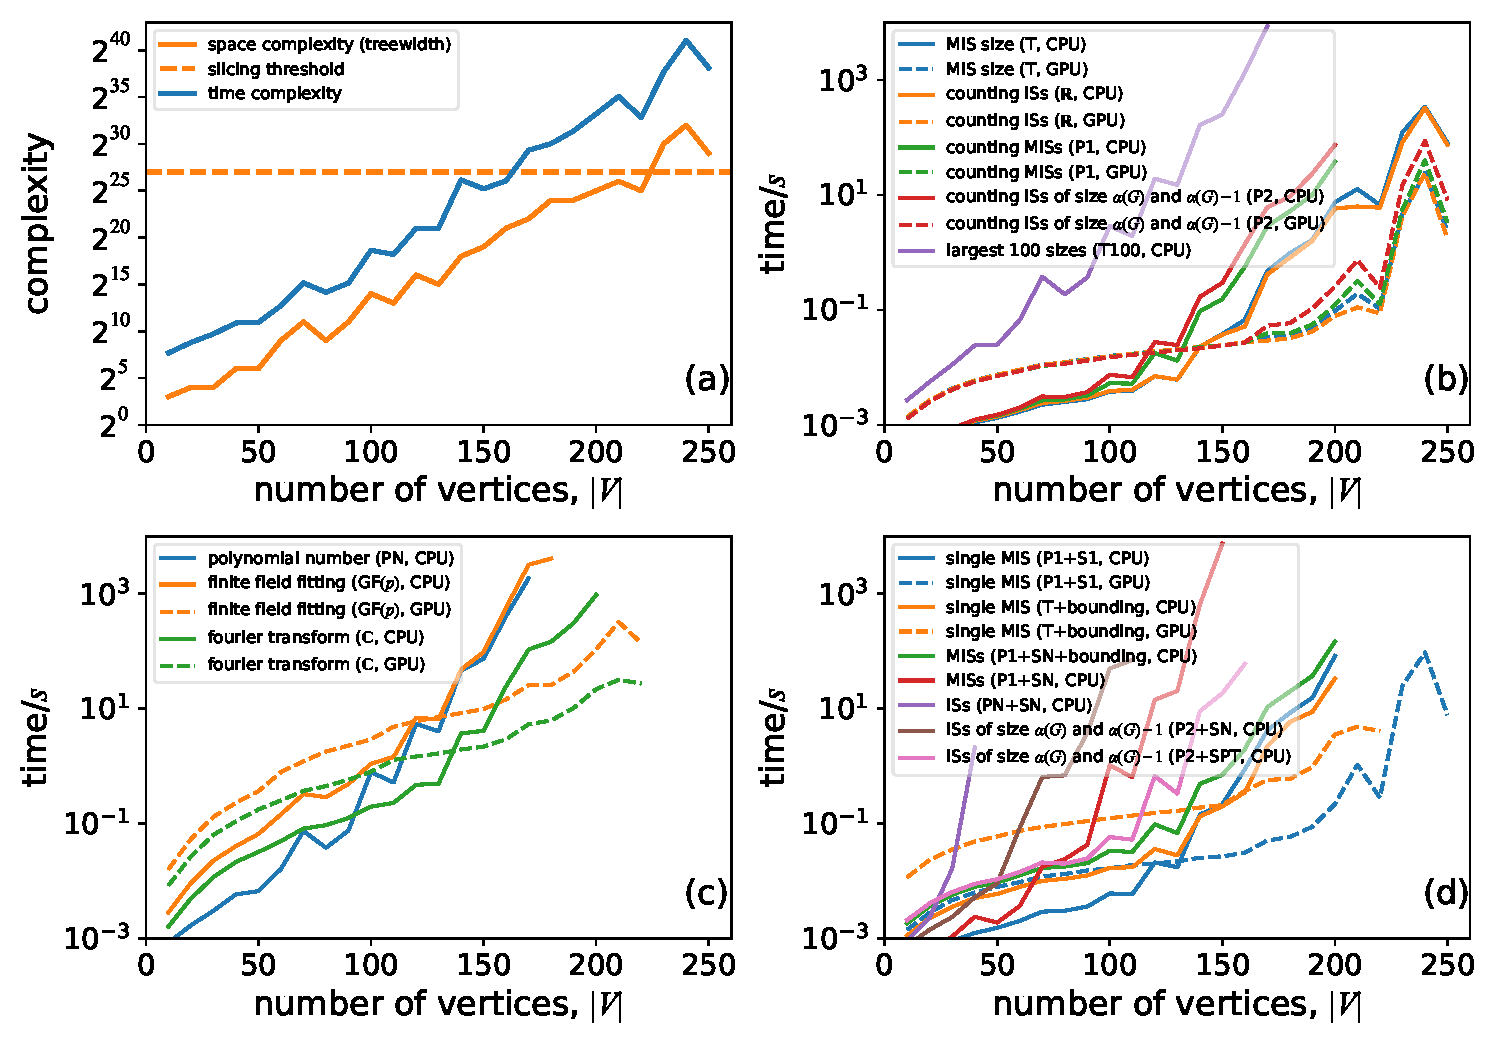
\includegraphics[width=\textwidth, trim={0cm 0cm 0cm 0cm}, clip]{figures/fig1.pdf}
    \caption{Benchmark results for computing different solution space properties of independent sets of random three-regular graphs with different tensor element types.
    The time in these plots only includes tensor network contraction, without taking into account the contraction order finding and just-in-time compilation time.
    Legends are properties, algebra, and devices that we used in the computation; one can find the corresponding computed solution space property in Table 1 in the main text.
    (a) time and space complexity versus the number of vertices for the benchmarked graphs.
    (b) The computation time for calculating the MIS size and for counting the number of all independent sets (ISs), the number of MISs,
        the number of independent sets having size $\alpha(G)$ and $\alpha(G)-1$, and finding $100$ largest set sizes.
    (c) The computation time for calculating the independence polynomials with different approaches.
    (d) The computation time for configuration enumeration, including single MIS configuration, the enumeration of all independent set configurations, all MIS configurations, all independent sets,
    and all independent set configurations having size $\alpha(G)$ and $\alpha(G)-1$.
    }
    \label{fig:benchmark}
\end{figure}

\Cref{fig:benchmark}(a) shows the time and space complexity of tensor network contraction for different graph sizes.
The contraction order is obtained using the local search algorithm in Ref.~\cite{Kalachev2021}.
If we assume our contraction-order finding program has found the optimal treewidth, which is very likely to be true, the space complexity is the same as the treewidth of the problem graph.
Slicing technique~\cite{Kalachev2021} has been used for graphs with space complexity greater than $2^{27}$ (above the yellow dashed line) to fit the computation into a 16GB memory.
One can see that all the computation times in \Cref{fig:benchmark} (b), (c), and (d) have a strong correlation with the predicted time and space complexity.
While in panel (d), the computation time of configuration enumeration and sum-product expression tree generation also strongly correlates with other factors such as the configuration space size.
Among these benchmarks, computational tasks with data types real numbers, complex numbers, or tropical numbers (CPU only) can utilize fast basic linear algebra subprograms (BLAS) functions.
These tasks usually compute much faster than ones with other element types in the same category.
Immutable data types with no reference to other values can be compiled to GPU devices that run much faster than CPUs in all cases when the problem scale is big enough.
These data types do not include those defined in \Cref{eq:polynomial}, \Cref{eq:set}, \Cref{eq:ext-tropical} and \Cref{eq:expr} or a data type containing them as a part.
In \Cref{fig:benchmark}(c), one can see the Fourier transformation-based method is the fastest in computing the independence polynomial,
but it may suffer from round-off errors (\Cref{sec:fft}). The finite field (GF$(p)$) approach is the only method that does not have round-off errors and can be run on a GPU.
In \Cref{fig:benchmark}(d), one can see the technique to bound the enumeration space in \Cref{sec:bounding} improves the performance for more than one order of magnitude in enumerating the MISs.
The bounding technique can also reduce the memory usage significantly, without which the largest computable graph size is only $\sim150$ on a device with 32GB main memory.

We show the benchmark of computing the maximal independent set properties on $3$-regular graphs in \Cref{fig:benchmark-maximal},
including a comparison to the Bron-Kerbosch algorithm from Julia package \href{https://github.com/JuliaGraphs/Graphs.jl}{Graphs}~\cite{Graphs}.
\Cref{fig:benchmark-maximal}(a) shows the space and time complexities of tensor contraction, which are typically larger than those for the independent set problem.
In \Cref{fig:benchmark-maximal}(b), one can see counting maximal independent sets are much more efficient than enumerating them, while our generic tensor network approach runs slightly faster than the Bron-Kerbosch approach in enumerating all maximal independent sets.

\begin{figure} 
    \centering
    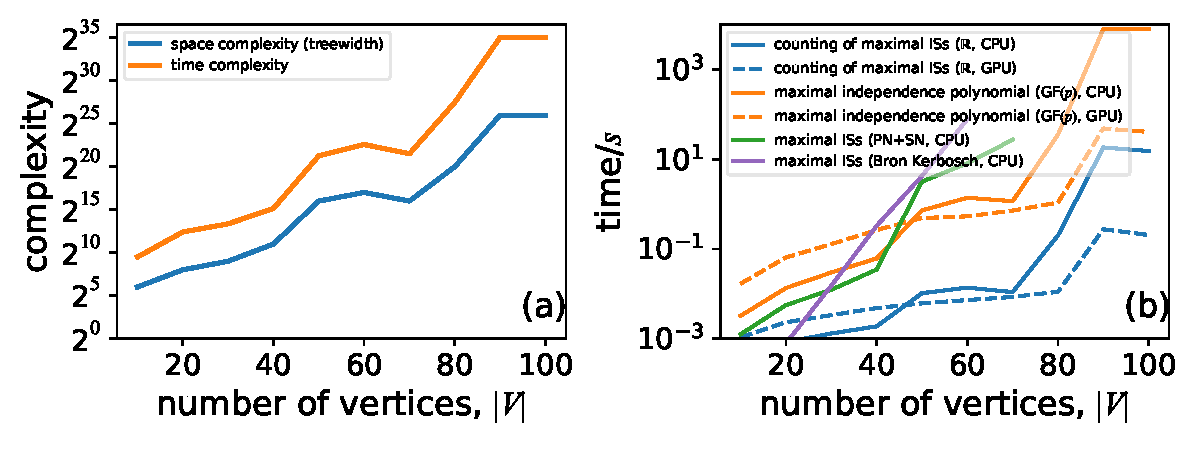
\includegraphics[width=\textwidth, trim={0cm 0cm 0cm 0cm}, clip]{figures/fig2.pdf}
    \caption{Benchmarks of computing different solution space properties of the maximal independent sets (ISs) problem on random three regular graphs at different sizes.
    (a) time and space complexity of tensor network contraction. 
    (b) The wall clock time for counting and enumeration of maximal ISs. % The missing data is due to the memory limit.
    }
    \label{fig:benchmark-maximal}
\end{figure}



\section{An example of increased contraction complexity for the standard tensor network notation}\label{sec:tensorbad}

In the standard Einstein's notation for tensor networks in physics, each index appears precisely twice: either both are in input tensors (which will be summed over) or one is in an input tensor and another in the output tensor.
Hence a tensor network can be represented as an open simple graph, where an input tensor is mapped to a vertex, a label shared by two input tensors is mapped to an edge and a label that appears in the output tensor is mapped to an open edge.
A standard tensor network notation is equivalent to the generalized tensor network in representation power.
A generalized tensor network can be converted to a standard one by adding a $\delta$ tensors at each hyperedge, where a $\delta$ tensor of rank $d$ is defined as
\begin{equation}
    \delta_{i_1, i_2,\ldots,i_d} = \begin{cases}
        1, & i_1=i_2=\ldots =i_d,\\
        0, & \text{otherwise}.
    \end{cases}
\end{equation}

In the following example, we will show this conversion might increase the contraction complexity of a tensor network.
Let us consider the following King's graph. \\

\centerline{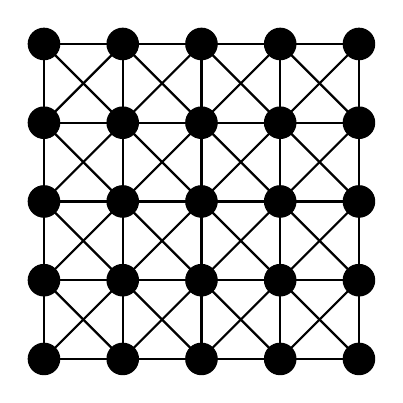
\begin{tikzpicture}
    \def\r{0.2}
    \foreach \x in {1,...,5}
        \foreach \y in {1,...,5}
            \filldraw[fill=black] (\x,\y) circle [radius=\r];
    \foreach \x in {1,...,5}
        \foreach \y in {1,...,4}{
            \draw [black,thick] (\x,\y) -- (\x,\y+1);
            \draw [black,thick] (\y,\x) -- (\y+1,\x);
        }
    \foreach \x in {1,...,4}
        \foreach \y in {1,...,4}{
            \draw [black,thick] (\x,\y) -- (\x+1,\y+1);
            \draw [black,thick] (\y+1,\x) -- (\y,\x+1);
        }
\end{tikzpicture}}

The generalized tensor network for solving the MIS problem on this graph has the following hypergraph representation, where we use different colors to distinguish different hyperedges.

\centerline{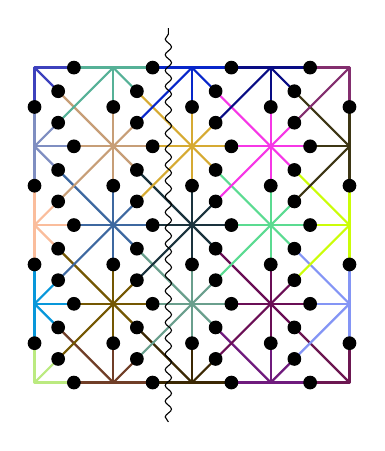
\begin{tikzpicture}
    \def\r{0.08}
    \def\a{0.07}
    \def\L{0.6}
    \def\l{0.1}
    \def\sql{0.24}
    \pgfmathsetseed{2}
    \foreach[evaluate={\cr=0.1+0.5*Mod(\x,2)}] \x in {1,...,5}
        \foreach[evaluate={\cg=0.1+0.3*Mod(\y,2); \cy=0.5-0.5*Mod(\y,2)}] \y in {1,...,5}{
            \edef\R{\pdfuniformdeviate 255}
            \edef\G{\pdfuniformdeviate 255}
            \edef\B{\pdfuniformdeviate 255}
            \xdefinecolor{MyColor}{RGB}{\R,\G,\B}
            \ifnum \x < 5
                \draw [thick, MyColor, opacity=1.0, line cap=round] (\x,\y) -- (\x+0.5,\y);
                \ifnum \y < 5
                \draw [thick, MyColor, opacity=1.0, line cap=round] (\x,\y) -- (\x+0.3,\y+0.3);
                \fi
                \ifnum \y > 1
                \draw [thick, MyColor, opacity=1.0, line cap=round] (\x,\y) -- (\x+0.3,\y-0.3);
                \fi
            \fi
            \ifnum \x > 1
                \draw [thick, MyColor, opacity=1.0, line cap=round] (\x,\y) -- (\x-0.5,\y);
                \ifnum \y < 5
                \draw [thick, MyColor, opacity=1.0, line cap=round] (\x,\y) -- (\x-0.7,\y+0.7);
                \fi
                \ifnum \y > 1
                \draw [thick, MyColor, opacity=1.0, line cap=round] (\x,\y) -- (\x-0.7,\y-0.7);
                \fi
            \fi
            \ifnum \y < 5
                \draw [thick, MyColor, opacity=1.0, line cap=round] (\x,\y) -- (\x,\y+0.5);
            \fi
            \ifnum \y > 1
                \draw [thick, MyColor, opacity=1.0, line cap=round] (\x,\y) -- (\x,\y-0.5);
            \fi
        }
    \foreach \x in {1,...,5}
        \foreach \y in {1,...,5}{
            %\filldraw[fill=black] (\x,\y) circle [radius=0.7*\r];
        }
    \foreach \x in {1,...,5}
        \foreach \y in {1,...,5}{
            \ifnum \y < 5
                \filldraw[fill=black] (\x,\y+0.5) circle [radius=\r];
                \filldraw[fill=black] (\y+0.5,\x) circle [radius=\r];
            \fi
        }
    \foreach \x in {1,...,4}
        \foreach \y in {1,...,4}{
            \filldraw[fill=black] (\x+0.3,\y+0.3) circle [radius=\r];
            \filldraw[fill=black] (\y+0.3,\x+0.7) circle [radius=\r];
        }
    \tikzset{decoration={snake,amplitude=.4mm,segment length=2mm,
                    post length=0mm,pre length=0mm}}
    \draw [decorate] (2.7, 0.5) -- (2.7, 5.5);
\end{tikzpicture}}
Vertex tensors are not shown here because they can be absorbed into an edge tensor and hence do not change the contraction complexity.
If we contract this tensor network in the column-wise order, the maximum intermediate tensor has rank $\sim L$, which can be seen by counting the number of colors at the cut.

By adding $\delta$ tensors to hyperedges, we have the standard tensor network represented as the following simple graph.

\centerline{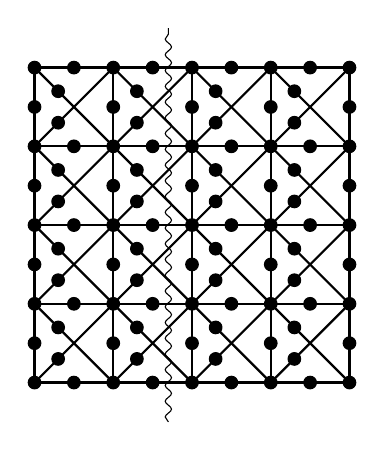
\begin{tikzpicture}
    \def\r{0.08}
    \def\a{0.1}
    \foreach \x in {1,...,5}
        \foreach \y in {1,...,5}
            \filldraw[fill=black] (\x,\y) circle [radius=\r];
    \foreach \x in {1,...,5}
        \foreach \y in {1,...,4}{
            \filldraw[fill=black] (\x,\y+0.5) circle [radius=\r];
            \filldraw[fill=black] (\y+0.5,\x) circle [radius=\r];
            \draw [black,thick] (\x,\y) -- (\x,\y+1);
            \draw [black,thick] (\y,\x) -- (\y+1,\x);
        }
    \foreach \x in {1,...,4}
        \foreach \y in {1,...,4}{
            \filldraw[fill=black] (\x+0.3,\y+0.3) circle [radius=\r];
            \filldraw[fill=black] (\y+0.3,\x+0.7) circle [radius=\r];
            \draw [black,thick] (\x,\y) -- (\x+1,\y+1);
            \draw [black,thick] (\y+1,\x) -- (\y,\x+1);
        }
    \tikzset{decoration={snake,amplitude=.4mm,segment length=2mm,
                    post length=0mm,pre length=0mm}}
    \draw [decorate] (2.7, 0.5) -- (2.7, 5.5);
\end{tikzpicture}}

In this diagram, the additional $\delta$ tensors can have ranks up to $8$.
If we still contract this tensor network in a column-wise order, the maximum intermediate tensor has rank $\sim3L$, i.e. the space complexity is $\approx 2^{3L}$, which has a larger complexity than using the generalized tensor network notation.

\section{The discrete Fourier transform approach to computing the independence polynomial}\label{sec:fft}

In \Cref{sec:finitefield} in the main text, we show that the independence polynomial can be obtained by solving the linear equation \Cref{eq:lineareq} using the finite field algebra.
One drawback of using finite field algebra is that its matrix multiplication is less computationally efficient compared with floating-point matrix multiplication.
Here, we show an alternative method with standard number types but with controllable round-off errors.
Instead of choosing $x_{i}$ as random numbers, we can choose them such that they form a geometric sequence in the complex domain $x_j = r\omega^j$, where $r \in \mathbb{R}$ and $\omega = e^{-2\pi i/( \alpha(G)+1)}$. The linear equation thus becomes
\begin{equation}
\left(\begin{matrix}
1 & r & r^2 & \ldots & r^{\alpha(G)} \\
1 & r\omega & r^2\omega^2 & \ldots & r^{\alpha(G)} \omega^{\alpha(G)} \\
\vdots & \vdots & \vdots &\ddots & \vdots \\
1 & r\omega^{\alpha(G)} & r^2\omega^{2{\alpha(G)}} & \ldots & r^{\alpha(G)}\omega^{{\alpha(G)}^2}
\end{matrix}\right)
\left(\begin{matrix}
a_0 \\ a_1 \\ \vdots \\ a_{\alpha(G)}
\end{matrix}\right)
= \left(\begin{matrix}
y_0 \\ y_1 \\ \vdots \\ y_{\alpha(G)}
\end{matrix}\right).
\end{equation}

Let us rearrange the coefficients $r^j$ to $a_j$, the matrix on the left side becomes the discrete Fourier transform matrix. Thus, we can obtain the coefficients by inverse Fourier transform $\vec a_r = {\rm FFT^{-1}}(\omega) \cdot \vec y$, where $(\vec a_r)_j = a_j r ^j$.
By choosing different $r$, one can obtain better precision for small $j$ by choosing $r<1$ or large $j$ by choosing $r>1$.

\section{Computing maximum sum combination}\label{sec:maxsum}
Given two sets $A$ and $B$ of the same size $n$.
It is known that the maximum $n$ sum combination of $A$ and $B$ can be computed in time $O(n\log(n))$.
The standard approach to solve the sum combination problem requires storing the variables in a heap --- a highly dynamic binary tree structure that can be much slower to manipulate than arrays.
In the following, we show an algorithm with roughly the same complexity but does not need a heap.
This algorithm first sorts both $A$ and $B$ and then uses the bisection to find the $n$-th largest value in the sum combination.
The key point is we can count the number of entries greater than a specific value
in the sum combination of $A$ and $B$ in linear time.
As long as the data range is not exponentially large, the bisection can be done in $O(\log(n))$ steps, giving the time complexity $O(n\log(n))$.
We summarize the algorithm as in \Cref{alg:sumcombination}.

\LinesNumberedHidden
\begin{algorithm}[!ht]
    \SetKwProg{Fn}{function}{}{end}
    \small
    \SetAlgoNoLine
    Let $A$ and $B$ be two sets of size $n$\;

    \tcp{sort $A$ and $B$ in ascending order}
    $A \gets {\rm sort}(A)$\;

    $B \gets {\rm sort}(B)$\;

    \tcp{use bisection to find the $n$-th largest value in sum combination}

    ${\rm high} \gets A_n+B_n$\;

    ${\rm low} \gets A_1+B_n$\;

    \While{true}{
        ${\rm mid} \gets ({\rm high} + {\rm low}) / 2$\;

        $c \gets \texttt{count\_geq}(n, A, B, {\rm mid})$\;

        \uIf{$c > n$}{
            ${\rm low} \gets {\rm mid}$\;
        }\uElseIf{$c = n$}{
            \Return \texttt{collect\_geq}$(n, A, B, {\rm mid})$\;
        }\Else{
            ${\rm high} \gets {\rm mid}$\;
        }
    }

    \Fn{{\rm \texttt{count\_geq}}($n$, $A$, $B$, $v$)}{
        $k \gets 1$\; \tcp*[l]{number of entries in $A$ s.t. $a+b\geq v$}

        $a \gets A_{n}$\; \tcp*[l]{the smallest entry in $A$ s.t. $a+b\geq v$}

        $c \gets 0$\; \tcp*[l]{the counting of sum combinations s.t. $a+b\geq v$}

        \For{$q$ = $n, n-1 \ldots 1$}{
            $b \gets B_{n-q+1}$\;

            \While{$k < n$ \textbf{and} $a+b \geq v$}{
                $k \gets k+1$\;

                $a \gets A_{n-k+1}$\;
            }

            \uIf{$a+b \geq v$}{
                $c \gets c + k$\;
            }\Else{
                $c \gets c + k-1$\;
            }
        }
        \Return c\;
    }

    % \Fn{\rm collect\_geq($n$, $A$, $B$, $v$)}{
    %     $k \gets 1$\; \tcp*[l]{number of entries in $A$ s.t. $a+b\geq v$}

    %     $a \gets A_{n}$\; \tcp*[l]{the smallest entry in $A$ s.t. $a+b\geq v$}

    %     $S \gets \{\}$ \tcp*[l]{the sum combinations s.t. $a+b\geq v$}

    %     \For{$q$ = $n, n-1 \ldots 1$}{
    %         $b \gets B_{n-q+1}$\;

    %         \While{$k < n$ \textbf{and} $a+b \geq v$}{
    %             $k \gets k+1$\;

    %             $a \gets A_{n-k+1}$\;
    %         }

    %         \uIf{$a+b \geq v$}{
    %             $m \gets k$\;
    %         }\Else{
    %             $m \gets k-1$\;
    %         }
    %         \For{$j$ = \KwTo $1,2\ldots,m$}{
    %             $S \gets S \cup \{b + A_{n-j+1}\}$
    %         }
    %     }
    %     \Return S\;
    % }
    \caption{Fast sum combination without using heap}\label{alg:sumcombination} 
\end{algorithm}

In this algorithm, function \texttt{collect\_geq} is similar the \texttt{count\_geq} except the counting is replace by collecting the items to a set.
Inside the function \texttt{count\_geq}, variable $k$ monotoneously increase while $q$ monotoneously decrease in each iteration and
the total number of iterations is upper bounded by $2n$.
Here for simplicity, we do not handle the special element $-\infty$ in $A$ and $B$ and the potential degeneracy in the sums.
It is nevertheless important to handle them properly in a practical implementation.

\section{Technical guides}\label{sec:technical}

This appendix covers some technical guides for efficiency, including an introduction to an open-source package \href{https://github.com/QuEraComputing/GenericTensorNetworks.jl}{GenericTensorNetworks}~\cite{GenericTensorNetworks} implementing the algorithms in this paper and the gist about how this package is implemented.
One can install \texttt{GenericTensorNetworks} in a Julia REPL, by first typing \colorbox{lightgray}{\texttt{]}} to enter the \texttt{pkg>} mode and then typing
\begin{lstlisting}
pkg> add GenericTensorNetworks
\end{lstlisting}
followed by an \colorbox{lightgray}{\texttt{<ENTER>}} key.
To use it for solving solution space properties, just go back to the normal mode (type \colorbox{lightgray}{\texttt{<BACKSPACE>}}) and type

\begin{lstlisting}
julia> using GenericTensorNetworks, Graphs

julia> # using CUDA

julia> solve(
           IndependentSet(
               Graphs.random_regular_graph(20, 3);
               optimizer = TreeSA(),
               weights = NoWeight(),
               openvertices = ()
           ),
           GraphPolynomial();
           usecuda=false
       )
0-dimensional Array{Polynomial{BigInt, :x}, 0}:
Polynomial(1 + 20*x + 160*x^2 + 659*x^3 + 1500*x^4 + 1883*x^5 + 1223*x^6 + 347*x^7 + 25*x^8)
\end{lstlisting}

Here the main function \texttt{solve} takes three inputs: the problem instance of type \texttt{IndependentSet}, the property instance of type \texttt{GraphPolynomial} and an optional key word argument \texttt{usecuda} to decide to use GPU or not.
If one wants to use GPU to accelerate the computation, ``\texttt{using CUDA}'' must be uncommented.
The problem instance takes four arguments to initialize: the only positional argument is the graph instance one wants to solve, the keyword argument \texttt{optimizer} is for specifying the tensor network optimization algorithm, the keyword argument \texttt{weights} is for specifying the weights of vertices as either a vector or \texttt{NoWeight()}, and the keyword argument \texttt{openvertices} is for specifying the degrees of freedom not summed over.
Here, we use the \texttt{TreeSA} method as the tensor network optimizer, and leave \texttt{weights} and \texttt{openvertices} as  default values. The \texttt{TreeSA} algorithm, which was invented in Ref.~\cite{Kalachev2021}, performs the best in most of our applications.
The first execution of this function will be a bit slow due to Julia's just-in-time compilation.
After that, the subsequent runs will be faster.
The following diagram lists possible combinations of input arguments, where functions in the \texttt{Graph} are mainly defined in the package \texttt{Graphs}, and the rest can be found in \texttt{GenericTensorNetworks}.

\centerline{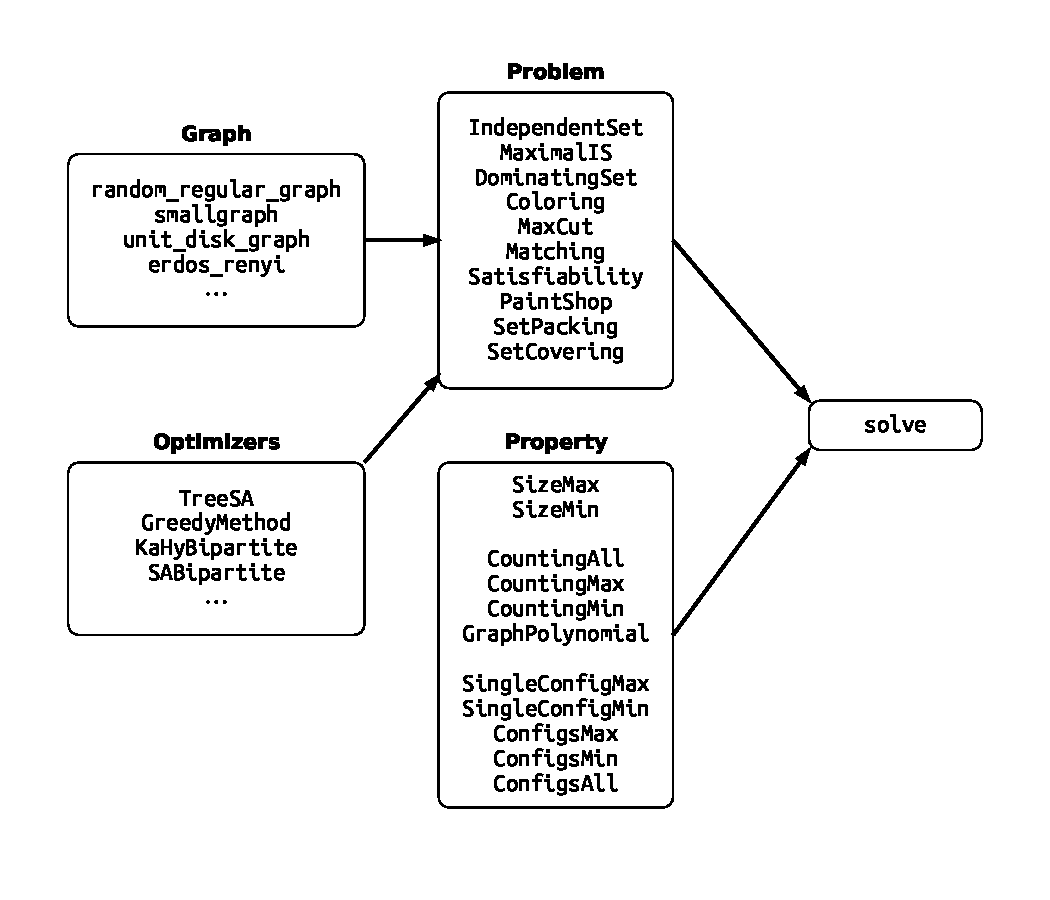
\includegraphics[width=0.8\textwidth, trim={0cm 1cm 0cm 1cm}, clip]{figures/fig7.pdf}}

The code we will show below is a gist of how the above package was implemented, which is mainly for pedagogical purpose.
It covers most of the topics in the paper without caring much about performance.
It is worth mentioning that this project depends on multiple open source packages in the Julia ecosystem:

\begin{description}
	\item[\href{https://github.com/under-Peter/OMEinsum.jl}{OMEinsum} and \href{https://github.com/TensorBFS/OMEinsumContractionOrders.jl}{OMEinsumContractionOrders}] are packages providing the support for Einstein's (or tensor network) notation and state-of-the-art algorithms for contraction order optimization, which includes the one based on KaHypar+Greedy~\cite{Gray2021, Pan2021} and the one based on local search~\cite{Kalachev2021}.
	\item[\href{https://github.com/TensorBFS/TropicalNumbers.jl}{TropicalNumbers} and \href{https://github.com/TensorBFS/TropicalGEMM.jl}{TropicalGEMM}] are packages providing tropical number and efficient tropical matrix multiplication.
	\item[\href{https://github.com/JuliaGraphs/Graphs.jl}{Graphs}] is a foundational package for graph manipulation in the Julia community.
	\item[\href{https://github.com/JuliaMath/Polynomials.jl}{Polynomials}] is a package providing polynomial algebra and polynomial fitting.
	\item[\href{https://github.com/scheinerman/Mods.jl}{Mods} and the \href{https://github.com/JuliaMath/Primes.jl}{Primes}] package providing finite field algebra and prime number manipulation.
\end{description}

They can be installed in a similar way to \texttt{GenericTensorNetworks}.
After installing the required packages, one can open a Julia REPL, and copy-paste the following code snippet into it.

\lstinputlisting[breaklines]{demo.jl}

\bibliographystyle{siamplain}
\bibliography{refs}
\end{document}
